\subsection{Handling linear-in-state aggregations}
\label{sec:linear-in-state-compilation}

We now consider the problems of detecting if an aggregation function is
linear-in-state and setting up auxiliary state for such linear-in-state
aggregation functions (Figure~\ref{fig:compiler-steps}). Recall that an
aggregation function is linear-in-state if the updates to all state variables
within the aggregation function can be written as $S =
\boldsymbol{A}(\mathbf{p}) \cdot S + \boldsymbol{B}(\mathbf{p})$).  A general
solution to this problem is challenging because the aggregation function can
take varied forms. For instance, the assignment $S = \frac{S^2 - 1}{S -1}$ is
linear-in-state, but detecting that it is linear-in-state needs the compiler to
perform algebraic simplifications.

We take a pragmatic approach and sacrifice completeness, but still cover useful
functions. Specifically, we only detect linear-in-state state updates through
simple syntactic pattern matching in the compiler (\ie without any algebraic
transformations).  Despite these simplifications, the \TheSystem compiler
correctly identifies all the linear-in-state aggregations in
Figure~\ref{fig:example-perf-queries} and targets the multiply-accumulate atom
that we added to the Banzai pipeline.

To describe how linear-in-state detection works, we introduce some terminology.
Recall that an aggregation function takes two arguments (\S\ref{sec:language}):
a list of state variables (\eg a counter) and a list of tuple fields (\eg the
TCP sequence number). We use the term variable in this subsection to refer to
either a state variable or a tuple field. These are the only variables that can
appear within the body of the aggregation function.\footnote{\TheSystem
supports local variables within the function body, but the more general
algorithm is not materially different from the simpler version we present
here.}

\begin{figure}
\centering
% Figure from
% https://docs.google.com/drawings/d/1Y-AC8YxCGkOJsaPILN_Fr1jKed1BKs0UdEab86r9T3g/edit?usp=sharing
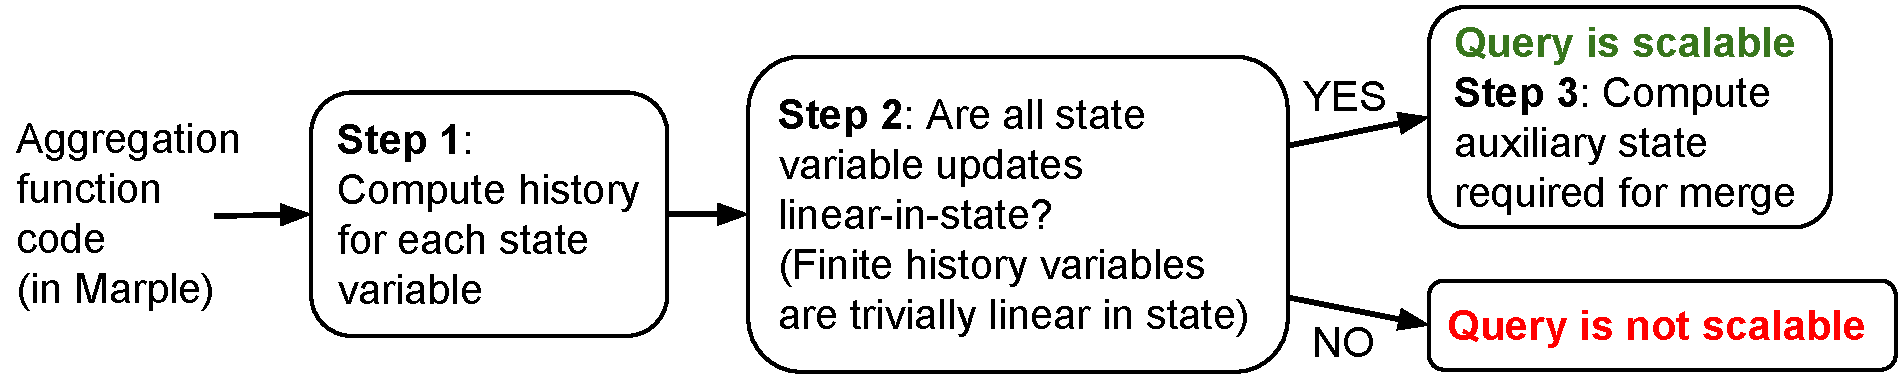
\includegraphics[width=\columnwidth]{pq_compiler-steps.pdf}
\caption{Steps for compiling linear-in-state updates.}
\label{fig:compiler-steps}
\end{figure}

%resume

We carry out a three-step procedure for linear-in-state
detection, summarized in \Fig{compiler-steps}.  First, for each variable in an
aggregation function we assign a {\em history}.  This history tells us how many
previous packets we need to look at to determine a variable's value accurately
(history = 1 means the current packet). For instance, for the value of a byte
counter, we need to look back to the beginning of the packet stream (history =
$\infty$), while for a variable that tracks the last TCP sequence number
we need to only look back to the previous packet (history = 2). Consistent with
the definition of history, constants are assigned a history value of 0, and
variables in the tuple field list are assigned a history of 1. For state
variables, we use \Alg{history} to determine each variable's history.

Second, once each variable has a history, we look at the history of each state
variable $s$. If the history of $s$ is a finite number $k$, then $s$ only
depends on the last $k$ packets and the state update for that variable is
trivially linear-in-state, by setting $A$ to 0 and $B$ to the aggregation
function itself.\footnote{More precisely, the parts of the aggregation function
that update $s$.} If $s$ has an infinite history, we use syntactic pattern
matching to check if the update to $s$ is linear-in-state.

Third, if all state variables have linear-in-state state updates, the
aggregation function is linear-in-state, and we generate the auxiliary state
that permits merging of the aggregation function (\S\ref{sec:aggregation}). If
not, we use the set of stateful instructions developed in Domino~\cite{domino_sigcomm}
to implement the aggregation function. We now describe each of the three steps
in detail.

\Para{Determining history of variables.} To understand \Alg{history}, observe that if all
assignments to a state variable only use variables that have a finite history,
then the state variable itself has a finite history. For instance, in
\Fig{running-example-code}, right after it is assigned, {\ct lastseq} has a history of 1 because it only
depends on the current packet's fields {\ct tcpseq} and {\ct payload\_len}. To
handle branching in the code, \ie {\ct if (predicate) \{...\}} statements, we
generalize this observation. A state variable has finite history if  (1) it 
has finite history in all its assignments in all branches of the program,
and (2) each branching condition {\ct predicate} itself only depends on
variables with a finite history.

Concretely, {\sc computeHistory} (line \ref{line:computeHistoryStart}) assigns each
variable a history corresponding to an upper bound on the number of past
packets that the state variable depends on. We track the history separately for
each branching {\em context}, \ie the sequence of branches enclosing any
statement.\footnote{Currently, \TheSystem forbids multiple {\ctfoot if ...
else} statements at the same nesting level; hence, the enclosing branches
uniquely identify a code path through the function. This restriction is not
fundamental; the more general form can be transformed into this form.} The
algorithm starts with a default large pessimistic history (\ie an approximation
to $\infty$) for each state variable (line \ref{line:curr-hist-init}), and
performs a fixed-point computation (lines
\ref{line:fixed-point}--\ref{line:fixed-point-end}), repeatedly iterating over
the statements in the aggregation function (line
\ref{line:fp-agg-begin}--\ref{line:fp-agg-end}).

For each assignment to a state variable in the aggregation function, the
algorithm updates the history of that state variable in the current branching
context (lines \ref{line:stmt-iteration}--\ref{line:stmt-history-update}). For
each branch in the aggregation function, the algorithm maintains a new
branching context and a history for the branching context itself (lines
\ref{line:encounter-branching}--\ref{line:branch-ctx-update-end}).  At the end
of each iteration, the algorithm increments each variable's history to denote
that the variable is one packet older (line \ref{line:inc}).  The algorithm
returns a conservative history $k$ for each state variable, including possibly
max\_bound (line \ref{line:curr-hist-init}, \Alg{history}) to reflect an
infinite history.

\begin{small}
\begin{algorithm}
  \caption{Determining history of all state variables}
  \label{alg:history}
  \begin{algorithmic}[1]
    \State hist = \{state = \{true: max\_bound\}\} \Comment{Init.
      hist. for all state vars.} \label{line:curr-hist-init}
    \Function{computeHistory}{{\cta fun}}\label{line:computeHistoryStart}
    \While{hist is still changing} \Comment{Run to fixed point.}\label{line:fixed-point}
    \State hist $\gets$ \{\}
    \State ctx $\gets$ true \Comment{Set up outermost context.}
    \State ctxHist $\gets$ 0 \Comment{History value of ctx.}
    \For{stmt in {\cta fun}} \label{line:stmt-iteration} \label{line:fp-agg-begin}
    \If{stmt == {\cta state = expr}}
    \State hist[state][ctx] $\gets$ {\sc getHist}(ctx, expr,
    ctxHist) \label{line:stmt-history-update}
    \ElsIf{stmt == {\cta if predicate}}\label{line:encounter-branching}
    \State save context info (restore on branch exit)\label{line:branch-ctx-update-start}
    \State newCtx $\gets$ ctx \textbf{and} predicate
    \State ctxHist $\gets$ {\sc getHist}(ctx, newCtx, ctxHist)
    \State ctx $\gets$ newCtx\label{line:branch-ctx-update-end}
    \EndIf
    \EndFor \label{line:fp-agg-end}
    \For{ctx, var in hist}\Comment{Make history one pkt older.}
    \State hist[var][ctx] $\gets$ min(hist[var][ctx] + 1, max\_bound)\label{line:inc}
    \EndFor
    \EndWhile \label{line:fixed-point-end}
    \EndFunction
    \Function{getHist}{ctx, {\cta ast}, ctxHist}
    \For{{\cta xi} $\in$ {\sc leafNodes}({\cta ast})}\label{line:used-var-start}
    \State hi = hist[{\cta xi}][ctx]
    \EndFor\label{line:used-var-end}
    \State \textbf{return} max(h1, ... , hn, ctxHist) \label{line:assign-max-hist}
    \EndFunction
  \end{algorithmic}
\end{algorithm}
\end{small}

Now we show precisely how the histories are updated as each statement of the
aggregation function is processed using the helper function {\sc getHist}.
Consider a statement assigning a variable to an expression, {\ct x = expr},
within a branching context {\ct ctx}. Then the history of {\ct x} is the
maximum of the history of the predicates in {\ct ctx} and the history of the
expression {\ct expr}. This is because if either is a function of the last $k$
packets, then {\ct x} is a function of at least the last $k$ packets.  To
determine the history of {\ct expr}, suppose the AST of {\ct expr} contains the
variables {\ct x1, x2, ..., xn} as its leaves. Then, the history of {\ct expr}
is the maximum of the histories of the {\ct xi}.  For example, the history for
{\ct lastseq} after its assignment in {\ct oos\_count} is the maximum of 1
({\ct tcpseq} and {\ct payload\_len} are functions of the current packet), and
0 (for the enclosing outermost context {\ct true}).

%The fixed-point iterations converge because the assigned state histories in a
%context are non-increasing.
%

\Para{Determining if a state variable's update is linear-in-state.} For each
state variable $S$ with an infinite history, we check whether the state updates
are linear-in-state as follows: (1) each update to $S$ is syntactically affine,
\ie $S \gets A \cdot S + B$ with either $A$ or $B$ possibly zero; and (2) $A$,
$B$ and every branch predicate depend on variables with a finite history. This
approach is sound, but incomplete: it misses updates such as $S = \frac{S^2 -
1}{S - 1}$.

\Para{Determining auxiliary state.} For each state variable with a
linear-in-state update, we initialize four pieces of auxiliary state for a
newly inserted key:\footnote{This can happen either when a key first appears or
reappears following an eviction.} (1) a running product $S_A = 1$; (2) a packet
counter $c = 0$; (3) an entry log, consisting of relevant fields from the first
$k$ packets following insertion; and (4) an exit log, consisting of relevant
fields from the last $k$ packets seen so far.  After the counter $c$ crosses
the packet history bound $k$, we update $S_A$ to $A \cdot S_A$ each time $S$ is
updated.\footnote{This stateful update itself can be implemented through a
multiply-accumulate atom.} When the key is evicted, we send $S_A$ along with
the entry and exit logs to the backing store for merging (see Appendix~\ref{app:merge}).
